\specialchap{序言}

随着物理学的发展,人们对于世界的理解也越来越深入。在粒子物理相关研究中,组成世界的基本粒子一共有 12 种,分为 6 种夸克,3 种带电轻子以及 3 种中微子。随着对于这十二种粒子的深入研究和理解,人们在量子场论的框架下基于量子色动力学和弱电相互统一理论,构建了标准模型(Standard Model, SM)。标准模型成功解释了宇宙中物质的构成以及它们之间的相互作用,并被大量实验所证实。2012 年标准模型所预测的最后一种粒子——希格斯玻色子的发现,更是完美地符合了标准模型的预测。

在标准模型所描述的基本粒子中,中微子显得十分地神秘和特殊。对中微子的研究最早可以追溯到 1930 年,奥地利物理学家泡利(Wolfgang Ernst Pauli)在一封解释 $\beta$ 衰变能谱连续问题的信中,首次提出$\beta$衰变可能会产生一种微小的电中性粒子。随后这个假设被费米(Enrico Fermi)引入到了他的 $\beta$ 衰变理论中\supercite{wilson1968fermi}。1956 年,随着 Clyde Cowan 和 Frederick Reines 在实验中首次确认了电子中微子的存在\supercite{cowan1991detection},人们才开始了解这一神秘的基本粒子。$\mu$ 中微子于1962年被Brookhaven国家实验室发现\supercite{danby1962observation},而后直到 2000 年,最后一种中微子 $\tau$ 中微子存在的直接证据才被费米实验室找到\supercite{kodama2001observation}。

在标准模型中中微子是没有质量的,但是大量过去和进行中的中微子实验,如超级神冈(Super-Kamiokande)\supercite{fukuda1998evidence},萨德伯里中微子观测站(SNO)\supercite{ahmad2002direct}等,都观测到了中微子震荡现象。在对于该现象的诸多解释中,最为自然的是中微子并非如标准模型所预言的质量为零,而是拥有一个很小的质量。这一理论可能标志着在标准模型之外,未被探索的新物理的存在。

中微子既然可能有质量,它质量的来源便是一个十分有趣的问题。如果假设中微子是狄拉克费米子(Dirac fermions),那么为了使它产生微小的质量,中微子与希格斯场相互作用的耦合系数会比夸克等其它粒子小12个量级,如此巨大的差别令人难以信服。另一种假设是中微子是马约拉纳费米子(Majorana fermions),即它自身是自己的反粒子。相对而言这种模型更为自洽,但它也意味着标准模型中轻子数守恒的推断会被打破,也将为理论物理带来巨大的改变。然而到目前为止,还没有足够的实验观测能够判断哪种模型更为正确\supercite{zhoushun}。

在中微子到底是何种费米子的相关研究中,有一类实验致力于寻找被称作无中微子双 $\beta$ 衰变(NLDBD)\supercite{avignone2008double}的稀有事件。在标准模型中,有一些核素因为束缚能的原因不能发生单次 $\beta$ 衰变,但是它们可以通过一个次级的弱相互作用来同时释放出两个电子(正电子)和两个反中微子(中微子),如图\ref{fig:nldbd}(a) 所示,这种衰变模式被称作双 $\beta$ 衰变(Double beta decay, DBD)。双 $\beta$ 衰变事件虽然稀有,但它已经被实验所观测和证实。如果中微子是马约拉纳费米子,即中微子和反中微子是同一种粒子,那么双 $\beta$ 衰变中第一次释放出的反中微子(中微子)又可能作为中微子(反中微子)参与第二次衰变。对外体现为核素直接衰变出两个电子(正电子)而不产生反中微子(中微子),如图\ref{fig:nldbd}(b) 所示。这种现象就被称作无中微子双 $\beta$ 衰变事件。

\begin{figure}
    \centering
    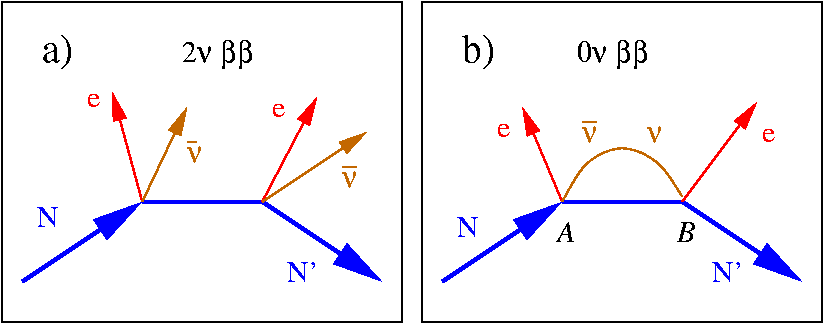
\includegraphics[width=0.5\columnwidth]{pic/nldbd.png}
    \caption{有中微子双 $\beta$ 衰变 (a) 以及无中微子双 $\beta$ 衰变 (b) 示意图。}
    \label{fig:nldbd}
\end{figure}

如果 NLDBD 事件被证实,那么不但意味着轻子数不再守恒,中微子的质量也可以通过其半衰期计算得到,如公式\ref{eq1}所示\supercite{avignone2008double},其中 $G^{0\nu}$ 是相空间因子,$M^{0\nu}$ 是核矩阵元素。从公式中可以看出,如果 NLDBD 事件的半衰期 $T^{0\nu}_{1/2}$ 已知,那么可以通过公式求得马约拉纳中微子质量 $\langle m_{\beta\beta}\rangle$ 。中微子绝对质量量级和中微子的质量顺序也可以由 $\langle m_{\beta\beta}\rangle$ 进一步计算得到,从而加深人们对于中微子的认识和了解。

\begin{equation}
    (T_{1/2}^{0\nu})^{-1}=G^{0\nu}|M^{0\nu}|^2\frac{\langle m_{\beta\beta}\rangle ^2}{m_e^2}
    \label{eq1}
\end{equation}

近年来世界上很多实验组都在进行 NLDBD 事件的探测,根据2015年美国核科学顾问局的报告 \supercite{NLDBD_NSAC},现在正在进行的实验有CUORE\supercite{Artusa:2014lgv}, EXO-200\supercite{Albert:2014awa}, GERDA\supercite{Agostini:2016iid}, KamLAND-Zen\supercite{KamLAND-Zen:2016pfg}, Majorana\supercite{Abgrall:2013rze},SNO+\supercite{Andringa:2015tza} 等。目前最好的实验结果是 KamLAND-Zen 给出的 $^{136}$Xe NLDBD 半衰期 $T^{0\nu}_{1/2}>1.07\times10^{26}$ 年。在经过广泛的交流后,这些NLDBD实验组们达成了普遍的共识:至少需要 1 吨量级的放射性同位素才有可能通过探测 NLDBD 事件来确定中微子的质量顺序。为了顺利的达成这一实验目的,不仅仅需要能够顺利的生产出吨量级的放射性同位素,同时需要极佳的探测器分辨率和极低的本底噪声,以及鉴别 NLDBD 
和本底的方法。

粒子和天气物理氙探测器第三期实验(Particle And Astrophysical Xenon Experiment III,以下简称 PandaX-III )便是一个设计中的吨级 $^{136}$Xe 无中微子双 $\beta$ 衰变探测实验,它使用高压气氙时间漂移室(TPC)探测器,并将其放置于锦屏地下实验室来屏蔽宇宙射线本底。实验计划在两到三年内建立出第一个 200kg 级探测器。本文详细描述了 PandaX-III 实验设计和前期测试中模拟的相关工作,分为以下几个部分:第一章简单介绍了整个项目;第二章描述了探测器背景模拟的相关工作;第三章介绍了使用深度神经网络 (Deep Neural Network, DNN) 中的卷积神经网络(Convolution Neural Network, CNN)来鉴别本底事件和信号。在 PandaX-III 实验模拟工作之外,本文第四章给出了使用 GPU 加速 Roofit 卷积的方法以解决在中微子能谱研究时探测器能量分辨率变化而造成难于拟合的问题。上述工作主要是本文作者完成的。PandaX-III 项目中探测器设计,电子学等其它相关工作的描述可以参见 PandaX-III 中期设计报告\supercite{cdr}。

% vim:ts=4:sw=4